\documentclass{article}\usepackage[]{graphicx}\usepackage[]{xcolor}
% maxwidth is the original width if it is less than linewidth
% otherwise use linewidth (to make sure the graphics do not exceed the margin)
\makeatletter
\def\maxwidth{ %
  \ifdim\Gin@nat@width>\linewidth
    \linewidth
  \else
    \Gin@nat@width
  \fi
}
\makeatother

\definecolor{fgcolor}{rgb}{0.345, 0.345, 0.345}
\newcommand{\hlnum}[1]{\textcolor[rgb]{0.686,0.059,0.569}{#1}}%
\newcommand{\hlsng}[1]{\textcolor[rgb]{0.192,0.494,0.8}{#1}}%
\newcommand{\hlcom}[1]{\textcolor[rgb]{0.678,0.584,0.686}{\textit{#1}}}%
\newcommand{\hlopt}[1]{\textcolor[rgb]{0,0,0}{#1}}%
\newcommand{\hldef}[1]{\textcolor[rgb]{0.345,0.345,0.345}{#1}}%
\newcommand{\hlkwa}[1]{\textcolor[rgb]{0.161,0.373,0.58}{\textbf{#1}}}%
\newcommand{\hlkwb}[1]{\textcolor[rgb]{0.69,0.353,0.396}{#1}}%
\newcommand{\hlkwc}[1]{\textcolor[rgb]{0.333,0.667,0.333}{#1}}%
\newcommand{\hlkwd}[1]{\textcolor[rgb]{0.737,0.353,0.396}{\textbf{#1}}}%
\let\hlipl\hlkwb

\usepackage{framed}
\makeatletter
\newenvironment{kframe}{%
 \def\at@end@of@kframe{}%
 \ifinner\ifhmode%
  \def\at@end@of@kframe{\end{minipage}}%
  \begin{minipage}{\columnwidth}%
 \fi\fi%
 \def\FrameCommand##1{\hskip\@totalleftmargin \hskip-\fboxsep
 \colorbox{shadecolor}{##1}\hskip-\fboxsep
     % There is no \\@totalrightmargin, so:
     \hskip-\linewidth \hskip-\@totalleftmargin \hskip\columnwidth}%
 \MakeFramed {\advance\hsize-\width
   \@totalleftmargin\z@ \linewidth\hsize
   \@setminipage}}%
 {\par\unskip\endMakeFramed%
 \at@end@of@kframe}
\makeatother

\definecolor{shadecolor}{rgb}{.97, .97, .97}
\definecolor{messagecolor}{rgb}{0, 0, 0}
\definecolor{warningcolor}{rgb}{1, 0, 1}
\definecolor{errorcolor}{rgb}{1, 0, 0}
\newenvironment{knitrout}{}{} % an empty environment to be redefined in TeX

\usepackage{alltt}
\usepackage{amsmath} %This allows me to use the align functionality.
                     %If you find yourself trying to replicate
                     %something you found online, ensure you're
                     %loading the necessary packages!
\usepackage{amsfonts}%Math font
\usepackage{graphicx}%For including graphics
\usepackage{hyperref}%For Hyperlinks
\usepackage[shortlabels]{enumitem}% For enumerated lists with labels specified
                                  % We had to run tlmgr_install("enumitem") in R
\hypersetup{colorlinks = true,citecolor=black} %set citations to have black (not green) color
\usepackage{natbib}        %For the bibliography
\setlength{\bibsep}{0pt plus 0.3ex}
\bibliographystyle{apalike}%For the bibliography
\usepackage[margin=0.50in]{geometry}
\usepackage{float}
\usepackage{multicol}

%fix for figures
\usepackage{caption}
\newenvironment{Figure}
  {\par\medskip\noindent\minipage{\linewidth}}
  {\endminipage\par\medskip}
\IfFileExists{upquote.sty}{\usepackage{upquote}}{}
\begin{document}

\vspace{-1in}
\title{Lab 07 -- MATH 240 -- Computational Statistics}

\author{
  Ben Horner \\
  Colgate University  \\
  Math Department  \\
  {\tt email@domain}
}

\date{March 13, 2025}

\maketitle

\begin{multicols}{2}
\begin{abstract}
The beta distribution is useful in modeling probabilities, rates, and other proportion as it and it's key characteristics (mean, variance, skewness, excess kurtosis) are easily defined and calculated. However, when taking a sample of random data, we must estimate those key characteristics. Here, we seek to examine those estimations and compare them to the population-level statistics, find that an increase in sample size will result in the estimated value approaching the population-level. On top of that, the sampling distributions follow a normal distribution around the population-level value.
\end{abstract}

\noindent \textbf{Keywords:} Beta Distribution; Probability Density; Moments; Sample Size; Variation

\section{Introduction}
The beta distribution is a continuous distribution that is used to model a random variable X that ranges from 0 to 1. This makes it useful for modeling proportions, probabilities, or rates. The beta distribution is also known for being remarkably flexible with regards to its shape --- it can be left-skewed, right-skewed, or symmetric depending on the value of the parameters that define its shape: $\alpha > 0$ and $\beta > 0$. We can use these parameters alone to not only define the distribution, but calculate the mean, variance, skewness, and excess kurtosis. Additionally, using the centered and uncentered moments of the beta distribution is another way to calculate these population-level characteristics.

However, often times we may not have access to the beta, alpha, or moment of the distribution, and thus need to approximate it based off of the data. As such, we will examine whether data summaries help, is the sample size important, and also model the variation of the data summaries when compared to the population-level values. 


\section{Methods}
The mean, variance, skewness, and excess kurtosis of a distribution are key summary characteristics that tell us more about the data we are looking at. With a beta distribution, we can calculate the population-level values using either the $\alpha$ and $\beta$ or the moments. Throughout this process, we load and use the following libraries: \texttt{ggplot2} \citep{ggplot2} and \texttt{patchwork} \citep{patchwork} for plotting and visualizing data, \texttt{tidyverse} \citep{tidyverse} to manipulate and summarize data, and \texttt{e1071} \citep{e1071} and \texttt{cumstats} \citep{cumstats} for additional statistical functions and analysis. 

\subsection{Describing and Summarizing The Population}
As the beta distribution's probability density function is defined in terms of the parameters $\alpha$ and $\beta$, the population-level characteristics are similarly defined by them. Using a function we created to summarize the mean, variance, skewness, and excess kurtosis (hereafter referred to as key characteristics) and a function to plot a beta distribution, compared to a Gaussian, we considered four cases: 
Beta($\alpha = 2, \beta = 5$), Beta($\alpha = 5, \beta = 5$), Beta($\alpha = 5, \beta = 2$), and Beta($\alpha = 0.50, \beta = 0.50$). 
To confirm our function works, we also computed the population-level key characteristics via the moments of the beta distribution, which match those using alpha and beta.

\begin{knitrout}\scriptsize
\definecolor{shadecolor}{rgb}{0.969, 0.969, 0.969}\color{fgcolor}
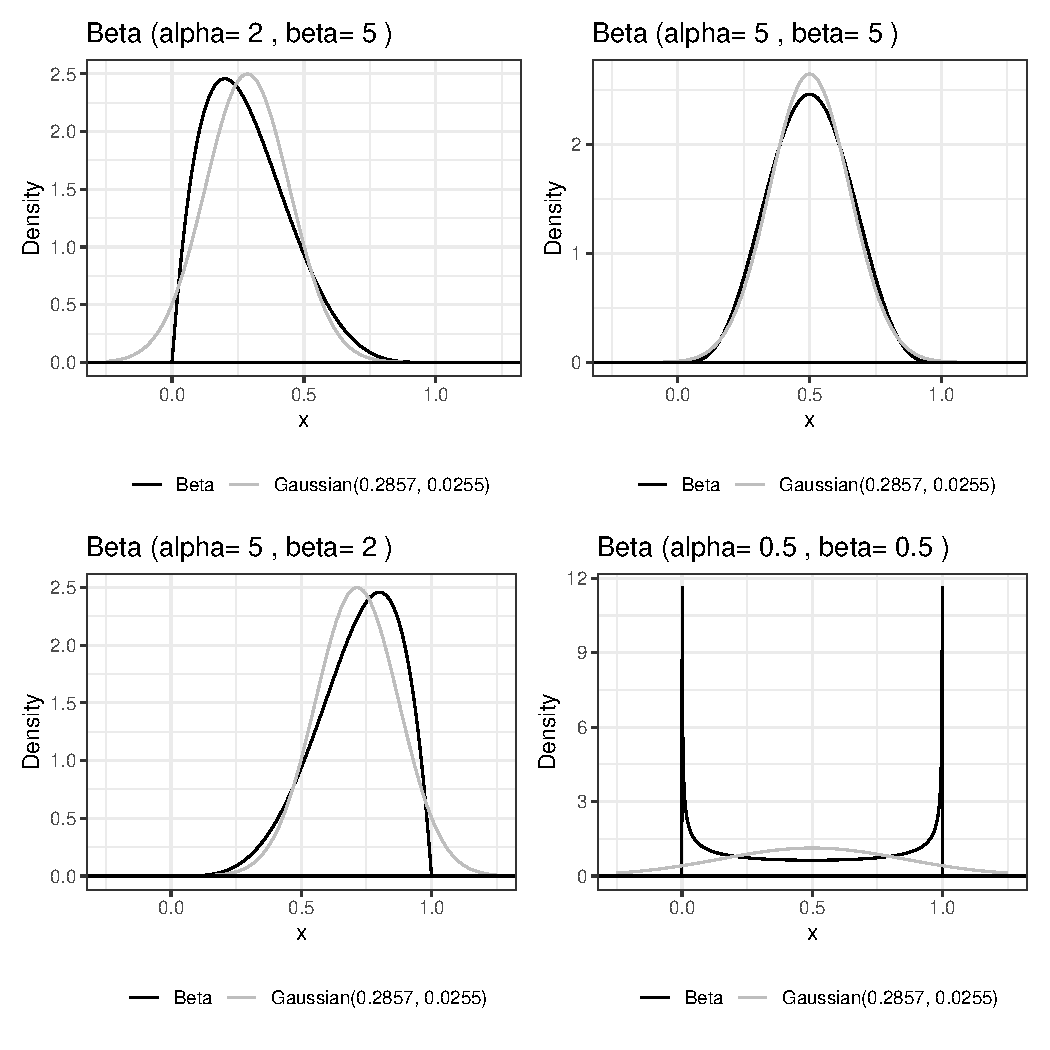
\includegraphics[width=\maxwidth]{figure/unnamed-chunk-1-1} 
\end{knitrout}

% latex table generated in R 4.4.2 by xtable 1.8-4 package
% Thu Mar 13 12:12:36 2025
\begin{table}[H]
\centering
\resizebox{\columnwidth}{!}{  % Resize the table to fit the text width
\begin{tabular}{rlrrrr}
  \hline
 & beta\_distribution & mean & varience & skewness & excess\_kurtosis \\ 
  \hline
1 & 2,5 & 0.29 & 0.03 & 0.60 & -0.12 \\ 
  2 & 5,5 & 0.50 & 0.02 & 0.00 & -0.46 \\ 
  3 & 5,2 & 0.71 & 0.03 & -0.60 & -0.12 \\ 
  4 & 0.5,0.5 & 0.50 & 0.12 & 0.00 & -1.50 \\ 
   \hline
\end{tabular}
} % End of resizebox
\caption{Summary of Beta Distribution Parameters}
\end{table}

\subsection{Summarizing Random Data}
When summarizing data, our goal is to approximate what the population distribution might be. We test this by generating a sample of $n = 500$ from each of the considered beta distributions using \texttt{set.seed(7272)} to ensure consistency across samples and attempts. We summarize the data using \texttt{summarize()} from \texttt{dplyr} \citep{tidyverse} and plot a histogram of the generated sample and its estimated density (red) compared to the population level beta function for the same alpha and beta (blue).
\begin{knitrout}\scriptsize
\definecolor{shadecolor}{rgb}{0.969, 0.969, 0.969}\color{fgcolor}
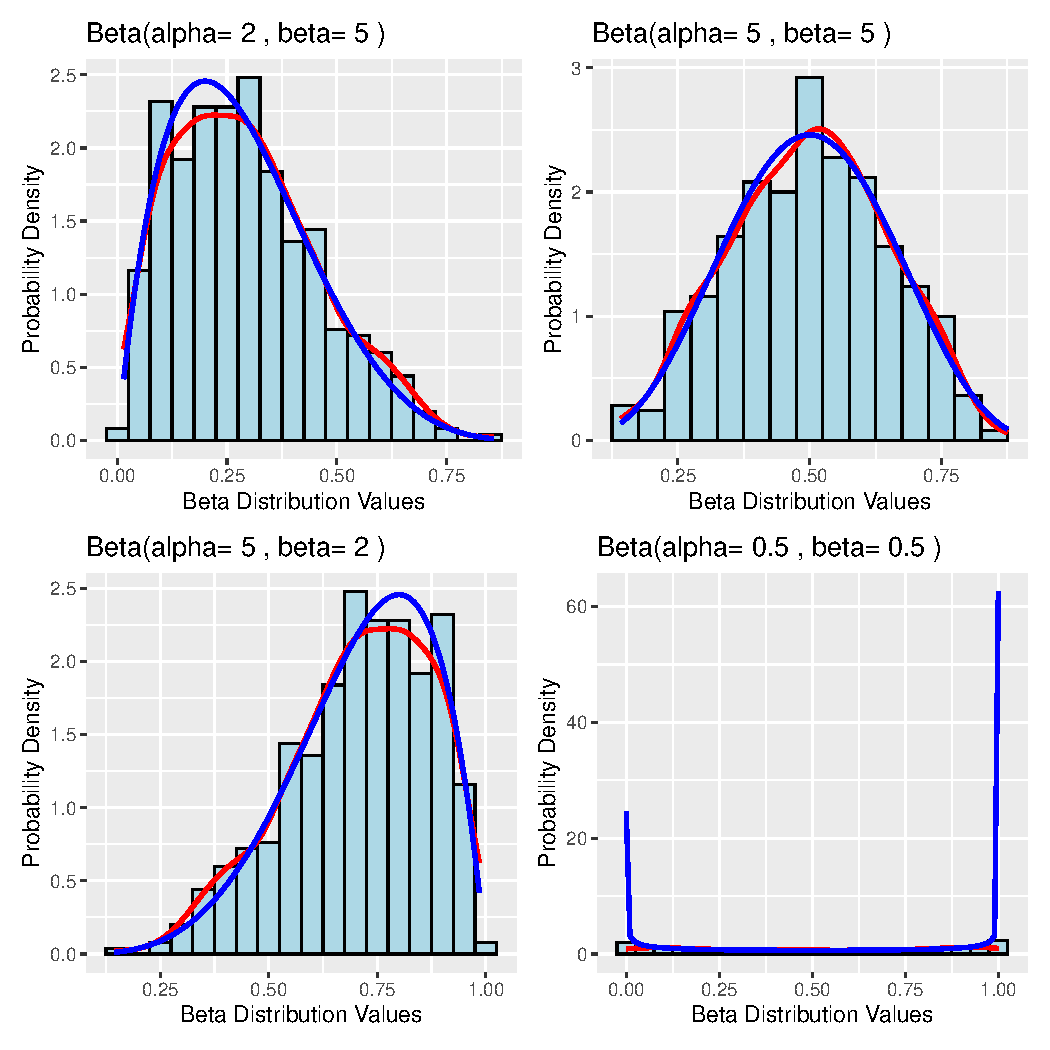
\includegraphics[width=\maxwidth]{figure/unnamed-chunk-2-1} 
\end{knitrout}

\subsection{Modeling Variation in Data Samples}
When taking a random sample of data, each sample varies from the last. As our goal is to model sampled data with a population-level distribution, we examine how our estimations of the key characteristics vary from sample to sample. Beginning with our set seed of 7272 to generate the random sample, we iterate $(1:1000)$ through seeds 7272+i, where i is the iteration. Our result is a sample of $n = 1000$ means, variances, skewnesses, and excess kurtosises, which we plot to examine their distribution.

\begin{knitrout}\scriptsize
\definecolor{shadecolor}{rgb}{0.969, 0.969, 0.969}\color{fgcolor}
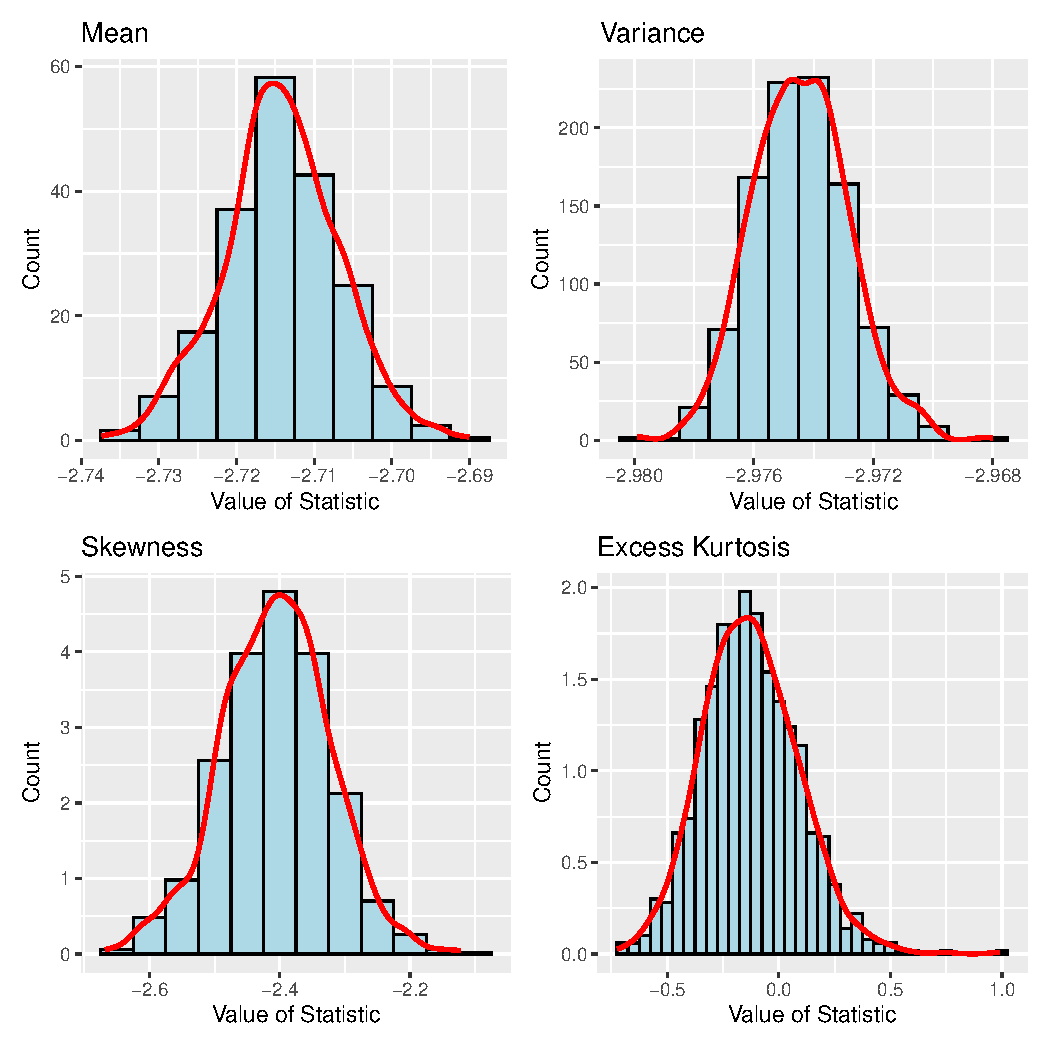
\includegraphics[width=\maxwidth]{figure/unnamed-chunk-3-1} 
\end{knitrout}


\section{Discussion}
When analyzing data, the key characteristics can provide essential summaries to guide one's research. However, often we only have a sample of the population instead of access to the true parameters of a distribution and as such, we estimate the key parameters. These summaries do help, and especially as the sample size increases, it approaches the true values for the population. Additionally, the sampling distribution of the beta function's key characteristics appear to follow normal (gaussian) distribution itself, with the standard deviation and spread of the sampling distribution increasing from the mean to varaiance, to skewness, and finally excess kurtosis. In the future, this will allow us to determine the accuracy of such estimated characteristics. 

%%%%%%%%%%%%%%%%%%%%%%%%%%%%%%%%%%%%%%%%%%%%%%%%%%%%%%%%%%%%%%%%%%%%%%%%%%%%%%%%
% Bibliography
%%%%%%%%%%%%%%%%%%%%%%%%%%%%%%%%%%%%%%%%%%%%%%%%%%%%%%%%%%%%%%%%%%%%%%%%%%%%%%%%
\vspace{2em}

\noindent\textbf{Bibliography:} Note that when you add citations to your bib.bib file \emph{and}
you cite them in your document, the bibliography section will automatically populate here.

\begin{tiny}
\bibliography{bib}
\end{tiny}
\end{multicols}


\end{document}
